\chapter{Least square regression, from small to big data}
\label{ch:least-square}

\section{Linear Regression at One Dimension}

Let us work at one dimension: $p =1$. If we work with N points, then
$i=1,\cdots,N$, and we work with a set of data $(x_i,y_i)$.

The goal here is to make a prediction of what the $y$ data should be when $x$ is
given.

The simplest possible model is the linear regression given by the equation 
\ref{linear1D}.

\begin{equation}
    y=\alpha + \beta x.
    \label{linear1D}
\end{equation}
Here, the main issue is to get the best $\alpha$ and $\beta$ for a partialicular
set of data. To know what the best choice is, we may define a cost function,
that returns a number representing how well the regression permorms. In neural
network problems, the cost fuction return number is associated with how well the
neural network performs in mapping training examples to the correct output.

There are several choices that can be made to define the cost function. At one
dimension, the simplest choice is the sum of squared residuals, defined in
equation \ref{SSR}, usually shortened as SSR.

\begin{equation}
    l(\alpha,\beta) = \nth \sumin (y_i - \alpha - \beta x_i )^2
    \label{SSR}
\end{equation} 

Figure \ref{fig1} illustrate a simple geometrical interpretation of what the SSR
is. Actually, the lower $\epsilon_i$, the better the fit.

\begin{marginfigure}
    \TODO
    \caption{geometrical intepretation of the SSR, where $\epsilon_i$ is given
        by the relation: $\epsilon_i^2 = (y_i - \alpha - \beta x_i)^2$}
    \label{fig1}
\end{marginfigure}

For all we have done up to now, we never have never worked with big data. We
need $p$ large enough to consider this as a real big data issue.

If we’re looking at a hundreds or thousands pixels picture, $p$ will be large
in comparison with $N$. That is a full statistics problem.

Currently, $p=1$ is small data, but all we did there has been a correct
introduction to clearly understand big data problems.

Striking a good fit necessitates finding the best $\alpha$ and the best $\beta$.
For this, we may look at the optimum, defined as the points where the derivative
of $l$ versus $\alpha$ and $\beta$ vanishes. This is given by equations
\ref{derlalpha} and \ref{derlbeta}.

\begin{eqnarray}
    \frac{\partial l}{\partial \alpha} & = & - \nth\sumin (y_i - \alpha - \beta x_i) = 0
    \label{derlalpha}\\
    \frac{\partial l}{\partial \beta} & =&  -\nth\sumin  x_i (y_i - \alpha -  \beta x_i) = 0
    \label{derlbeta}
\end{eqnarray}

To solve this set of equations, we require a substitution for $x$ and $y$.

Let’s define the mean values:
\marginnote{We must keep in mind that $\overline{x^2} \neq \bar{x}^2$.}
\begin{eqnarray}
    \bar{x} & = & \nth\sumin x_i\\
    \bar{y} & = & \frac{1}{N} \sum_{i=1}^N y_i\\
    \overline{xy} & =&  \frac{1}{N} \sum_{i=1}^{N} x_i y_i\\
    \overline{x^2} & =&  \frac{1}{N} \sum_{i=1}^N x_i^2
\end{eqnarray}

Thus, equations \ref{derlalpha} and \ref{derlbeta} can be reduced as:
\begin{eqnarray}
    \frac{\partial l}{\partial \alpha} &=& - (\bar{y} - \alpha - \beta \bar{x})
    \label{deralpha2}\\
    \frac{\partial l}{\partial \beta} &=& - (\overline{xy} - \alpha \bar{x} - \beta \overline{x^2})
    \label{derbeta2}
\end{eqnarray}

This yields to:

\begin{eqnarray}
    \alpha & = & \bar{y} + \beta \bar{x}\\
    \overline{xy} & = &  -\bar{y}\bar{x} - \beta \bar{x}^2 - \beta \overline{x^2}
\end{eqnarray}

\marginnote{We use the given notations:
    \begin{eqnarray*}
        \cov(x,y) &=& \bar{xy} - \bar{x}\bar{y} \\
        & =& \overline{(x-\bar{x})}(y-\bar{y}) \\
        \var(x) & =&  \cov (x,x) \\
        \sigma(x) & =& \sqrt{\var(x)}
    \end{eqnarray*}
}

There we may substitute $\alpha$ and $\beta$:

\begin{eqnarray*}
    \hat{\alpha} & =& \bar{y} - \hat{\beta}\bar{x}
\end{eqnarray*}

\begin{eqnarray*}
    \hat{\beta} & = & \frac{\overline{xy} - \bar{x}\bar{y}}{\overline{x^2} - \bar{x}^2} \\
    & = & \frac{\cov(x,y)}{\cov(x,x)}\\
    & =&  \frac{\cov(x,y)}{\var(x)}
\end{eqnarray*}


Let us define the Pearson coefficient $\mathcal{R}$ by the relation
\ref{pearson}.
\begin{equation}
    \mathcal{R} = \frac{\cov(x,y)}{\sigma(x) \sigma(y)}
    \label{pearson}
\end{equation}

The Pearson coefficient $\mathcal{R}$ is always comprised between $0$ and $1$.
Thus, we can define the quantity $\mathcal{R}^2$, that relates to the quality of
the fit:

\begin{equation}
    \mathcal{R}^2 = 1 - \frac{\hat{l}}{\var(y)}
\end{equation}


In the general case, we look at models where $\beta = 0$. In this case, the cost
function $l$ would be the sum of the square distance to the line.
Figure \ref{squaredistances} depicts two linear regressions with different
parameters. The right figure shows a much better linear regression, with
much lower square distances between the points and the line.

\begin{figure}
    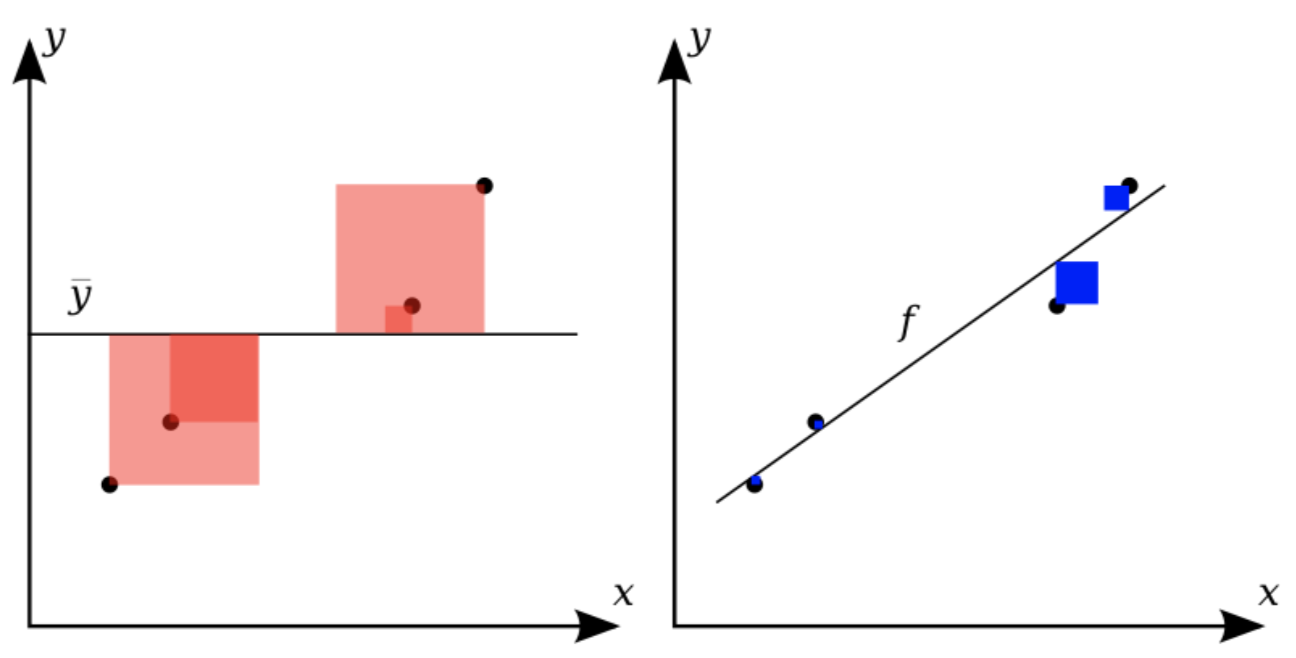
\includegraphics{./Figures/squaredistances.png}
    \caption{Two linear regression taken from two datasets. The left one shows higher square distances than the right one.}
    \label{squaredistances}
\end{figure}

We may note that in some cases, it would be better to rescale the axis to
fit the data with a linear regression. Logarithm axis is the most popular way
of rescaling an axis to have a correct assumption. It is usually more valuable
to rescale the axis and perform a linear regression, than trying to find an
higher order fit.

\section{Linear Regression at Higher Dimensions}

We are now considering higher dimensions data ($p>1$), that are full, meaning
that $p<<N$.
It means that, for an example of data, we might add different parameters. If we
take the example (given in class) of correlations between the velocity of people
versus the size of towns, we might add other relevant parameters, like the
average heigh of people, their ages, etc. We might then examine many potential
predictors. Thus we need to generalise the same things, where each input now
becomes a vector of p dimensions, as presented in equation \ref{pdim}

\begin{equation}
    (x_{i,1}, \cdots , x_{i,p}), \qquad \forall i
    \label{pdim}
\end{equation}

Let now $x_{i,j}$ be the matrix of the input data, where $i$ is the number of
samples, varying from 1 to $N$, and $j$ is the dimension, ranged between 1 to
$p$.

We may generalise the relation $\hat{y_i} = \hat{\alpha} + \hat{\beta}x_i$ in
the new \ref{gen2} equation: 

\begin{equation} 
    \hat{y_i} = \hat{\alpha} + \sum_{j=1}^p \hat{\beta_j} x_{ij}
    \label{gen2}
\end{equation}

If we have this key figure, we can always add 1 in the x vector, as the $p+1$
coordinate. We can thus assume that $\alpha$ vanishes. In fact, we can always
redefine the data so that $\alpha$ vanishes. We can also rescale the variable, by
removing the mean:

\begin{eqnarray}
x’&=& x-\bar{x}\\
y’&=& y-\bar{y}
\end{eqnarray}

Therefore, the output coordinate $\hat{y_i}$ can be written as the product
$\hat{y_i} = X \hat{\beta}$, that is a much more convenient way to write it.

That are just restrictions of the problems that help us to compute it.

Let $l(\beta)$ be the cross-function, define with equation \ref{lbeta}.

\begin{equation}
    l(\beta) = \frac{1}{N} \sum_{i=1}^N \left( y_i - \sum_{j=1}^p \beta_j x_{ij} \right)^2
    \label{lbeta}
\end{equation}

\marginnote{$^T$ denotes the transpose matrix, defined by the relation:
$\left[\mathbf{A}^\mathrm{T}\right]_{ij} = \left[\mathbf{A}\right]_{ji}$}

Let $Z$ be a vector whose components $z_i$ are defined as follows:

\begin{equation}
    \sum_{i=1}^N z_i^2 = ||Z||^2 = Z^TZ
\end{equation}

Therefore we can write the cross-function as:

\begin{equation}
    l(\beta) = \frac{1}{N} (Y-X\beta)^T(Y-X\beta)
\end{equation}

This form can easily be differentiated with $\beta$, and the retrieved derivative
vanishes at the extremum (eq. \ref{lextrem}).

\begin{equation}
    \frac{\partial l}{\partial \beta} =  -\frac{Z}{N} X^T(Y-X\beta) =0
    \label{lextrem}
\end{equation}

The equation \ref{lextrem} can be reduced as $X^TY = X^TX\beta$, which can be
solved by introducing the matrix $C = X^TX$ (eq. \ref{lextremC})\footnote{Note
    that 
\begin{equation*}
C_{ij} = \sum_{k=1}^N x_{kj} x_{ki}
\end{equation*}}

\begin{equation}
    \hat{\beta} = (X^TX)^{-1} X^TY = C^{-1} X^TY
    \label{lextremC}
\end{equation}

At higher dimension, the geometry consists in fitting with an hyperplane, as
shown on figure \ref{hyperplane}.

\begin{marginfigure}
    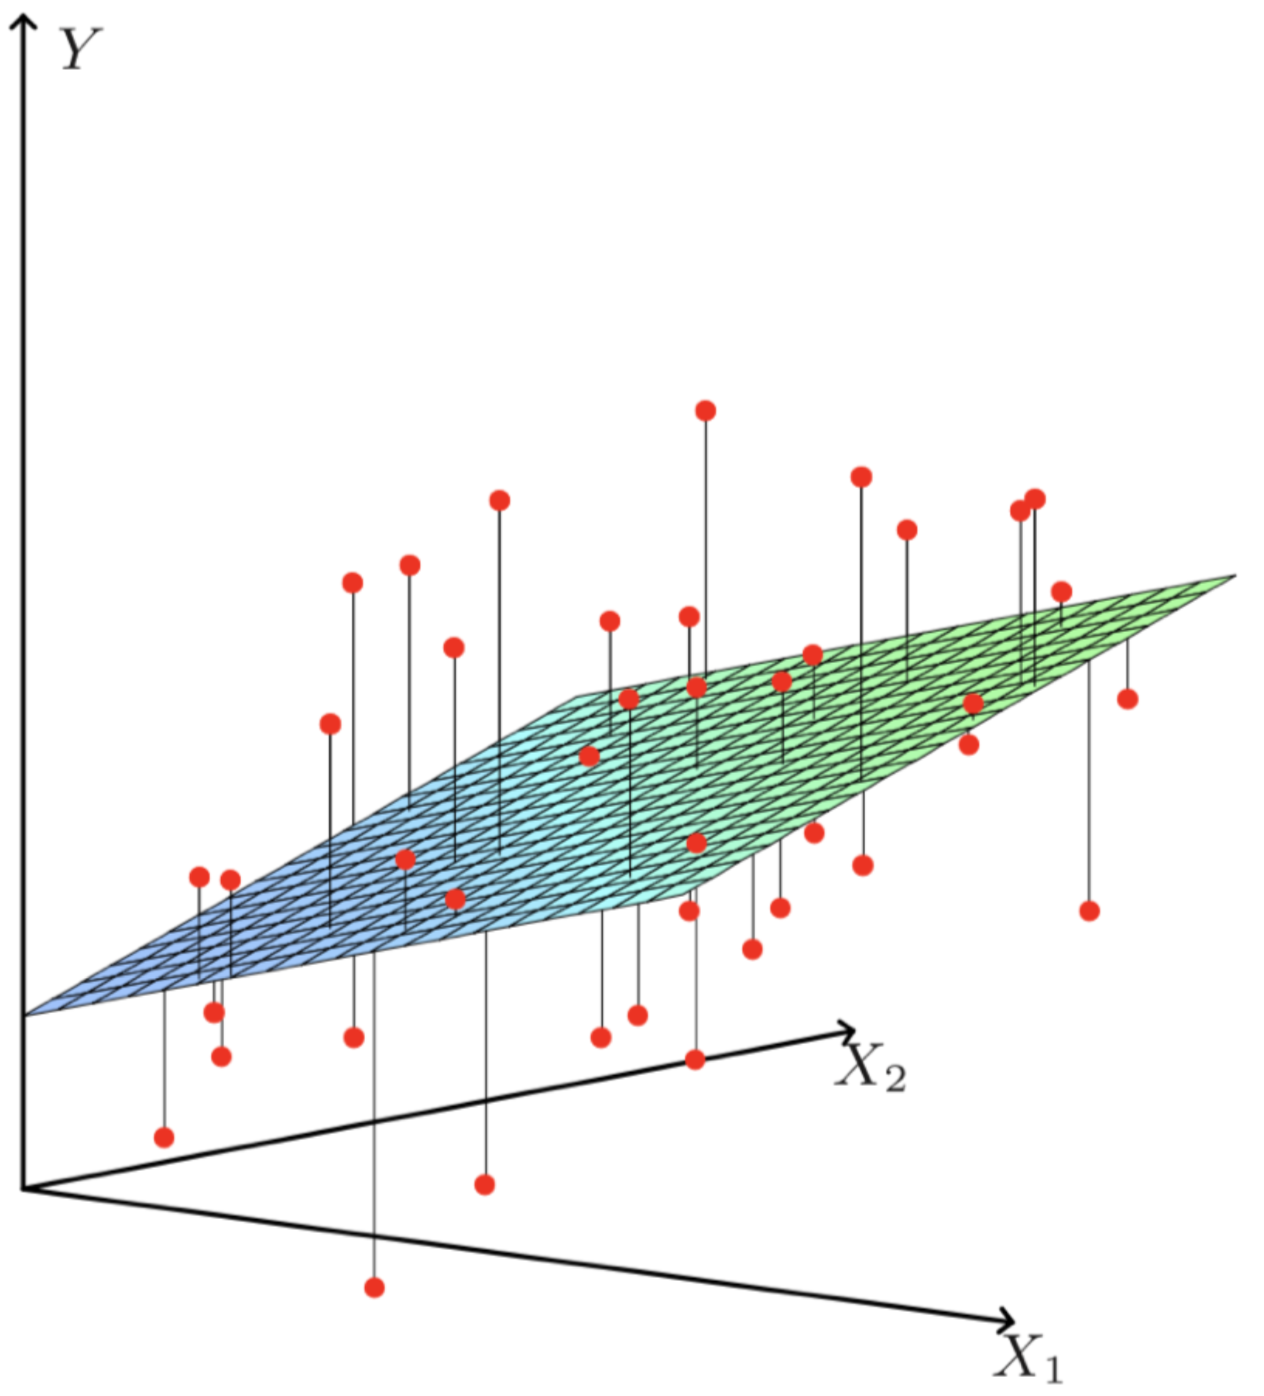
\includegraphics{./Figures/hyperplane.png}
    \caption{Linear least squares fitting with $X\in\mathbb{R}^2$. In this
        problem, we are looking for the linear function of X that minimises the
    sum of squared residuals from Y, which is an plane (hyperplane in dim 3)}
    \label{hyperplane}
\end{marginfigure}

Here, we are essentially solving a system of equations. We must consider the
number of variables adapted to the number of equations that we get. When there is
not enough equations (when $p$ is too small for example), the system is
undetermined. We cannot reduce it and do not have a single solution.

Actually, when $p>N$, we can solve this problem with the condition $\hat{l}=0$.
This is a situation where there are more parameters than there are equaltions. It
is easy to solve. The solutions consists in overfitting.

For instance if we have 100 parameters and 10 equations, we can never manage to
get any result. However, we can find easy solutions, but this will overfit.
At this stage, the system cannot be inverted.

When $p$ is large, even if it is of the same order of magnitude as $N$, we are
working with big matrixes, that can be tricky to invert with both proper
mathematical accuracy and computation performances. In such cases, we should
handle the data carefuly.

Large $p$ are typical way of using statistical learning methods, by
discriminating between datasets without having the aforesaid issues.
